\documentclass[11pt,a4paper]{article}
\title{Behaviour Analysis of Elderly using topic models}
\author{Kristin Rieping}
\usepackage[latin1]{inputenc} %andere lettertype
\usepackage{amsmath} %math symbols
\usepackage{amsfonts} %andere font maar wel math symbols
\usepackage{amssymb} % nog meer symbolen
\usepackage{graphicx} %plaatjes toevoegen
\usepackage{fullpage} %minder witte rand
\usepackage{cite} %voor het citeren

\begin{document}
\maketitle
\pagebreak
\tableofcontents
\pagebreak
%----------------------------------INTRODUCTION--------------------------------------------
\section{Introduction}
The world population increases unceasingly and thereby the percentage of elderly also increases. The manpower to take care of elderly is diminishing. So it becomes more and more important to give elderly the opportunity to live on there own and be more independent of health care. It is also important to monitor elderly in the case that they cannot live on their own anymore and to detect accidents automatically. While monitoring the behavior of elderly it might be possible to detect mental disorders.

New techniques give the possibility to monitor elderly from the distance or even automatically. Some of these techniques use cameras that are placed in the homes of elderly. But these methods are privacy-sensitive and often not adopted by the elderly.

Other methods use motion sensors that are placed at different locations in the homes of elderly. %find some example
Reading and interpreting this sensor data is often difficult and that is why often activity recognition is done to make the data more readable. But different approaches show that this is also a though challenge.
With many Machine Learning techniques it is also often the case that a lot of annotated data is required.  But the task of labeling a data set is time consuming and can also influence the output of the data while doing so. That is why unsupervised techniques are more preferable.\\



In this thesis we develop an unsupervised algorithm that detects patterns in the data automatically.
In a first step, which is inspired by~\cite{farrahi2008daily}, real live data is used to build a topic model. In a second step a genetic algorithm is used to find the best representation of the data according to the likelihood that is gained from the topic models found in the first step. 
From simple motion sensors we receive binary, time sequential data, that is gained over some period of time in the homes of elderly. There are a lot of sensors placed in the houses, which leads to highdimensional data, that is hard to interprete for classifying algorithms as well as for humans. A topic model in combination with a genetic algorithm might lead to a representation of the data that gives the opertunity to interprete the data more easily and also finds behaviour patterns in the data automatically. This furthermore makes it possible to detect deviations in the behaviour over a longer period of time. The data that we use is received in the same way as described in ~\cite{van2010activity}, except that our data is not annotated.\\

Topic models are usually used in the field of document classification. The idea is that every document might belong to a couple of different topics and a topic can be described with a distribution over words. A newly seen document can than be assigned to some topics according to the words that occure in the document. The document is than described with a distribution of topics. The topics of a model can be found in an unsupervised manner.
We use this idea to find topics in the given sensor data. So that a day in a persons life can be described with a distribution over topics. And a topic will be described with a distribution over observations. An example of a topic might be 'going to the toilet' or a more global example is 'getting up early'.\\
Our data differs from the data that is normally used for this kind of models in some way. For text classification the 'bag-of-words' model is often used. This model is not so easily applicable to the given sensor data, because of the multidimensional and the continous description of the data. A Text document usually does or does not contain a word of a given dictionary. Therefore our data needs to be descritized in some way.\\
In a first approach we first simply count the amount of times that a sensor is triggered in a certain window of time. This still produces a brought varity of observations and that is why we cluster the observations with k-means, so that we are able to use the topic model 'Latent Dirichlet Allocation' described in~\cite{blei2003latent}, on our data.\\
This approach has some drawbacks and therefore we develop a topic model based on LDA that models the clusters in the model itself with a Gaussian distribution in every dimension of the observation. In this way the topic model is able to handle high dimensional data. The model paramters are found with an EM-procedure, which uses the likelihood of the model to converge to the optimal model parameters.\\
\\
In the second part of the thesis we use a genetic algorithm to find the best representation of the data.
Earlier we described the part of descretizing the data in some way. Choosing the correct length of a timeinterval, in which the sensor activities are count, might be hard. There are also plenty of other variables to choose, that lead to a different representation of the data. For example we can choose to group all sensors together that are in the same room of the house. But we cannot be sure that this leads to a beter representation of the data. Further there are different kind of sensors placed in the houses and we might want to distinguish between these sensors, so that a different weigth is given while counting an activity. For example an activity at a door sensor might give more information of a persons behaviour then a motion sensor, which is triggered more often also by small, not that important movements. It might also a good idea to look at the transition of the observations, so given an observation, what are the observations before and after this one.\\
So the representation of the data depends from a lot of different variables. This variables are optimized with a genetic algorithm. The loglikelihood, from the previously derived topic models, is used as the fitness function of the genetic algorithm.\\

In the next chapter of this thesis we give an overview of related approaches. In section \ref{sec:DataDesc} we describe the data that we use in more detail. This is followed by section \ref{sec:TopicModels} which describes the two different ways of the usage of Topic Models with our data. In section \ref{sec:features} we describe the different ways of feature representation of our data and also show how the genetic algorithm is used. The section \ref{sec:Experiments} we describe the different experiments that we perfomed. We finalize the thesis with the section \ref{sec:DisCon}.


%  Instead of a bag-of-word model that describes our data, every observation is model with a Gaussian Distribution in every dimension.
% 
% 
% In a second step a genetic algorithm is used to find the best feature representation of the data. The data is discretized in times-slices and divided into different fields. The likelihood of the EM-algorithm of the topic model is used as a fitness function. In this way the best representation of the data can be found.\\ 
% Ik weet nog niet hoe ik dat precies doe, dus maar nog niet meer omschrijven.
% Together this two steps might give a good indication how this kind of data can be efficiently used with other machine learning techniques.
% This data also might give valuable information to health proffesionals. The topics described in the first step might give a good indication of the health of the elderly.
% 
% It might be possible to predict the health of a person and give additinal health care if needed.


\section{Related Work}
Articles:\\
-die ene\\
-die andere


%--------------------------------DATADESCRIPTION--------------------------------------------
\section{Data Description}
\label{sec:DataDesc}
\subsection{Sensors}
There are two different types of sensors installed in the homes. Reed and motion. Plaatjes ervan en hoe het is geinstaleerd is.
omschrijven hoe de twee sensoren werken. reed alleen als een deur wordt geopend en motion elke minuut weer kijken of er beweging is.
Er zijn wel wat problemen
niet altijd even betrouwbaar. Uitval van sensor. Soms twee keer aan/uit achterelkaar gevuurd.
two types of sensors installed
hoe ziet de data eruit wat zijn problemen ermee (continu tijdstippen met sensor aan/uit)
The sensors that are placed in the homes are placed at different locations, for example at doors, cupboards, microwave, toilet flush or several other places that a frequently used.
The sensors can have the values 0 and 1. If a sensor is activated it gets the value 1 and 0 if it is deactivated.
\subsection{Homes and persons}
The homes looks like shown in figure ... There might be small differences of the locations of the sensors due to the personal arrangements of peoples stuff.
The persons that live in the homes are people that need healthcare. The data is gained of in total five different people. The amount of data differs for every person.
there are five people
The houses look the same
the amount of data varies for every person
Wat zijn het voor mensen
Hoe ziet hun woning uit
waar zijn deze sensoren in de woning(weet ik dat??)
\subsection{Received Data}
An example of the data is shown in figure ... Here an hour of a typical day is plotted. 
The sensors are annotated and devided in five fields. The fields are ...
Wat is de data die we krijgen
wat zijn de sensor namen geplaatst zijn

 Several sensors are grouped together and form a field. In the following descriptions we use five fields, which are $\{$'kitchen','living room','bathroom','bedroom','hallway'$\}$
The sensors that define a field are specified manually.
From the sensors we receive the time when it is triggered and in which value it changes to. Possible values are $\{$0,1$\}$. In figure~\ref{fig:PlaineSensorData} an example of the sensor data over one day is shown.\\

\begin{figure}[h!]
  \centering
    	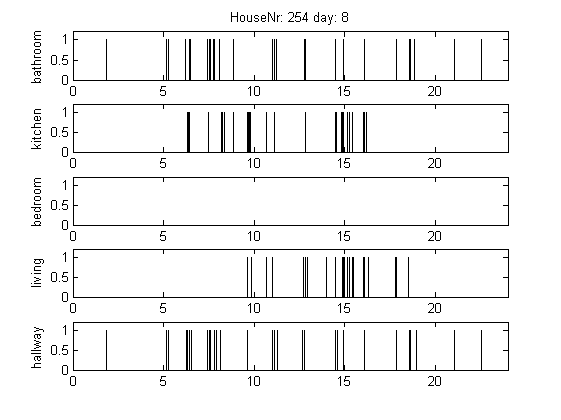
\includegraphics[width=0.7\textwidth]{Pictures/plainDataExample.png}
    \caption{Sensor Data for one day with five fields}
    \label{fig:PlaineSensorData}
\end{figure}












\pagebreak
%-----------------------------------TOPICMODEL----------------------------------------------
\section{Topic Models}
\label{sec:TopicModels}
In the Introduction of this section we describe the general idea of topic models followed by a section that describes how this kind of models can be used on the Sensor data that we have. Then we describe the approach with the combination of k-means clustering and the LDA model. And in the last part of this section we introduce the extension of the LDA model which combines the clustering and topic estimation in one algorithm.

\subsection{Introduction to Topic Models}
Een voorbeeld geven me documenten en woorden en topics. Hier ook LDA Blei model in tonen.
Neem een set van Newsarticelen. Er bestaan verschillende topic zo als politics, economy. This topics are characterized by several words and between topics there might be overlap between words that characterize a topic, but the distribution over words give a good indication to which topic a document belongs. Further one document might contain multiple different topics. So for example an article about Obama who speaks about the economic grow belongs for some part to the topic 'politics' and also to the topic 'economy'. And there might be several other topics that are included in such an article. Now the words that are contained in the article gives the indication about which topic are included in the article.\\
The model shown in figure is a way to capture the topics given a set of data (Corpus). Every  

\subsection{Topic models with Sensor Data}
Topic models are often used in the field of document classification. Given a set of documents (Corpus) it is assumed that every document belongs to one or more topic(s). So for example a news article may belong for some percentage to the topic 'Economy' and also for some percentage to the topic 'Politics'. Every topic can be described with a distribution of words. So if some specific words occur in a news article it is an indication that the article belongs to a certain topic.\\
We use this idea to find topics in our sensor data. To make use of topic models we first introduce the different levels of description given our data and relate them to the terms of document classification.
\begin{itemize}
 \item \textbf{Dataset/Corpus}: One dataset $C$ describes the sensor data that is gained in the home of one person. So every person has his own Dataset. This can be compared with a Corpus in document classification.
 \item \textbf{Day/Document}: Every Dataset is devided in days. A day can be compared with one document in a Corpus.
 \item \textbf{Observations/Words}: Finally every day is build of a set of observations. The amount and dimension of the observations depends on the representation of the features, which is described later in chapter \ref{sec:features}. Observations can be roughly compared with words in document classification.
\end{itemize}




There are some differences between the data used for topic detection in documents and our sensor data. The main difference is that words that look similar to each other, like ``illusion'' and ``allusion'', may belong to a totally different topic in the document classification. But in our case, two observation that are similar to each other, are more likely to refer to the same topic. So for example if the topic ``preparing food'' has the observation using fridge 3 times in it, an observation of using fridge 4 times may also refer to the same topic. So we cannot simply make use of the bag-of-word model on our data.

Another main difference is that in the topic model, that we want to use, it is assumed that the order of the words, in that they appear in the text, does not matter. In our case the time when an observation is made is of big influence. We can adjust this problem by adding an additional dimension for time to our observations. But this brings also some disadvantages with it while modeling, which is explained in the next chapter.


In the next two sections we describe the two different ways how we use the topic models with our data. First we describe the combination of k-means clustering and the basic LDA model as it is described in [Blei]. And after that we describe our new approach that combines the clustering and topic modelling in one algorithm. In this algorithm we step away from the bag-of-words model representation of the data.
 Nog toevoegen dat we twee manieren gaan gebruiken(LDAbasic and LDAext)
%%TOT HIER!


\subsection{K-means clustering and LDA}
 Now we first describe how the data is clustered and then we describe how we can use the LDA model on our data with the clustered found in the first step.

  \subsubsection{K-means}
 In the previous section we addressed the problem of a wide variance of observations. With a bag-of-words model, as it is used in the LDA approach, similar looking words/observations are not likely to be put in the same topic. All observations, that are not exactly the same, are independent from each other and may not lead to the same topic. Because of the low amount of training data it is not very likely that the same observation will be seen often enough to learn topics from the data properly.
That is why we need to reduce the amount of unique observations and group similar observations together. In terms of document classification, we could say that we need to reduce the size of the dictionary.

%TOT HIER

This is done with k-

In a first-approach we use k-means clustering to reduce the size of the dictionary, which is the set of all observations that can be found in the data.
We do not use the time dimension for the clustering part, because this would compromise our data so that clusters are not detected properly. We use the euclidean distance to determine the best mean.

maybe preprocess the data with coarse grain time dimension

size of the dictionary
is it the case that with a lot of data simialar looking words will be put in the same topic? Or will it just be a different topic?



In our data the size of the dictionary, which contains all unique observations in the whole corpus is relative large with respect to the size of the data that we have. There are a lot of different observations that are similar to each other, but differ only in one value of the 6 dimensions. So for example the observation $o_1=\{1 ,2 ,5 ,3,14\}$ is similar to the observation $o_2=\{2 ,2 ,5 ,3,14\}$. The only difference of sensor activities is in the first field. In the LDA model these two observations/words will be seen as two different dimensions and the similarities are not captured. In fact a lot of words will only be seen once in the whole corpus and finding good parameters is not possible.
 So we need to find a way to capture similar observations to build a proper topic model. A simple way is to cluster all observations together and then use the EM-algorithm to estimate the parameters of the  LDA model.
 For the clustering part we used the k-means algorithm. We reduced the size of the dictionary to 20. After that we use the EM-algorithm as described above.
 In the clustering we leave out the time dimension because this is fucking up the clusters
 
  \subsubsection{Latent Dirichlet Allocation with clustered Data}
The generative model 'Latent Dirichlet Allocation' [Blei] is a way to describe a topic model. In this model it is assumed that a Corpus can be generated from a distribution of topics, where every topic can be represented with a distribution of words. In our case the documents are days and the words are observations $o_n$. In the previous section we described how we reduced the size of the dictionary $V$.
The generative process that would create the data will look like this:

For every day that will be generated:
\begin{enumerate}
 \item Set the amount of observations in every document to size N (for every day the same amount).
 \item Choose a topic distribution $\theta \sim Dir(\alpha)$ for the day.
 \item For each of the N observations $o_n$:
 
 \begin{enumerate}
  \item Choose a topic $z_n \sim Multinomial(\theta)$.
  \item Choose a set of obeservations $o_n$ from the set of all observations $V$ from $p(o_n |z_n;\beta)$, a multinomial probability conditioned on the topic $z_n$. Where $\beta$ is the distribution over observations given a topic.
 \end{enumerate}

\end{enumerate}
%!!!Describe the model variables!!!!!

With the assumption that the data that we got from the sensor system has the same structure than the data created with the generative process we can find the model parameters $\alpha$ and $\beta$ for LDA with the EM-algorithme described in \cite{blei2003latent}.

\subsection{Extension to the LDA model}
In this section we explain how the part of clustering is combined within the LDA model itself. Instead of the k-means clusters we use a gaussian distribution to model every dimension within the features.


  \subsubsection{Motivation and Assumptions of the Model}
  
  In the previous section we clustered the data first with k-means and then used the LDA model to determine the topics of the model. This approach has some drawbacks. First of all the clusters that are found with k-means have a hard separation lines between the clusters. No quality measurement on the clusters is given and every point that falls in the cluster belongs to the cluster with the same probability, no matter how far it is away from the mean. Also every cluster has the same weight so there is no distinction between the clusters.

  With a Gaussian Mixture Model we might be able to distinguish between more or less important clusters. But we might want to let the topic model decide which topics have more influence and which not according to the data.\\
That is why we combined the clustering part and the topic estimation into one step. Instead of a multinomial distribution over the bag-of-words model of the observations given a topic, we model a Gaussian distribution over every dimension of the observations. In this way similar observation can be captured in the model itself and are not generalized in a cluster.\\
The difference is that instead of a large, fixed set of unique observations (Dictionary), with a multinomial distribution, instead we take a Gaussian distribution over every dimension of the observations. In this way smoothing is not necessary, because unseen observations will be handeled properly.
In the next sections we describe the model in more detail. We first give an overview of the generative process. Then we explain the variational inference that is necessary to make the parameter estimation possible. And finaly explain the EM-algorithm that determines the parameters.

Every topic will have its own distribution over the dimensions. A
topic can be described as shown in figure %\ref{fig:topic}.
In this figure an example of a topic description is shown
% \begin{figure}
%  \includegraphics[\width=\textwidth]{Pictures\topics.png}
%  \caption{An awesome topic}
%  \label{fig:topic}
% \end{figure}

  \subsubsection{Model description}
   meer uit de zicht het bestaat en het wordt niet gegenereerd.
  
  Our model assumes that every day in a dataset can be represented as random mixtures of latent topics, where every topic can be described as a distribution over observations. We assume the following generative procss for every day $m$ in $M$:
\begin{enumerate}
 \item The amount of observations on a day $m$ is fixed with size $N$ (for every day the same size).
 \item A distribution over the topics $\theta \sim Dir(\alpha)$ for that day.
 \item For each of the N observations $o_n$:
 
 \begin{enumerate}
  \item Estimate the topic $z_n \sim Multinomial(\theta)$.
  \item An obeservations $o_n$ is generated from $p(o_n |z_n,\boldsymbol\mu,\boldsymbol\sigma)$, a probabilty which can be drawn from a set of Gaussian distributions, which are conditioned on the dimension $d$ of the observation and the topic $z_n$. $\boldsymbol\mu$ and $\boldsymbol\sigma$ are two matrices of size  $D\times k$, which represent the mean and standard variance of the Gaussian distribution.
 \end{enumerate}

\end{enumerate}
  
In this model the amount of topics $k$ is assumed to be known and fixed and with it the size of the topic variable $z$.
 Here is the gaussian shit varibale description.
The probability for the observations is parameterized with two matrices $\boldsymbol\mu$ and $\boldsymbol\sigma$, both of size $D\times k$, where $D$ is the amount of dimensions in an observation and $k$ the amount of topics. They present the mean and standard deviation respectivally and for every topic $i$ and every dimension $d$ there is a set of parameters, which describes a Gaussian distribution.  Every value of a dimension for an observation $o_{ndi}$ can then be drawn from a Gaussian Distribution $\mathcal{N}(\mu_{di},\sigma_{di})$.
The size of the dimension $D$ is assumed to be fixed and a more extensive description of the representation of the observations is given in section \ref{sec:features}. $\alpha$ represents the Dirichlet parameter and is vector of length $k$.
Alpha beter uitleggen
the variable $\alpha$ represents the Dirichlet Parameter
$\alpha$ is a vector of length $k$.
Misschien hier ook het grafische model. Of toch misschien al eerder? Nee denk het niet, want als je het model alleen ziet dan weet je niet wat alles betekend. Dus het grafische model moet nu komen.

Given the parameters $\alpha$, $\mu$ and $\sigma$, the joint distribution of a topic mixture $\theta$, a set of $N$ topics $z$ and a set of $N$ observations $o$ is given by:
\begin{equation}
 p(\theta,\textbf{z},\textbf{w}|\alpha,\mu,\sigma) = p(\theta|\alpha) \prod_{n=1}^N p(z_n|\theta) p(w_n|z_n,\mu,\sigma)
\end{equation}


A visualization of this model is shown in figure \ref{fig:modelExt}.

\begin{figure}[t!]
\centering
\def\svgwidth{0.8\textwidth}
\input{Pictures/ModelExt.pdf_tex}
\caption{Graphical representation of the LDA model}
\label{fig:modelExt}
\end{figure}


  
Assuming that the generative process described above can describe the available data properly, we now want to find the parameters so that the model best describes our data. We want in fact maximize the probability for the dataset $C$ given the model with respect to the parameters $\alpha$, $\mu$ and $\sigma$. This probability looks like this
\begin{equation}
p(C|\alpha,\mu,\sigma) = \prod_{m=1}^M p(m|\alpha,\mu,\sigma)
\end{equation}
where $M$ is the amount of days within the dataset and the probability for a day $m$ given the three parameters, which is the marginal distribution over a day, is
\begin{equation} 
p(m|\alpha,\mu,\sigma) = \int p(\theta|\alpha)  \left( \prod_{n=1}^N \sum_{z_n} p(z_n|\theta) p(w_n|z_n, \mu,\sigma)  \right) d\theta
\end{equation}
This distribution is gained by integrating the joint distribution by $\theta$.
In the next section we describe how we find the optimal parameters.



  
  \subsubsection{Variational Inference}
 
  Thie marginal distribution can be written in terms of the parameter $\alpha$, $\mu$ and $\sigma$ as
  \begin{equation}
   p(m|\alpha,\mu,\sigma) = \frac{\Gamma (\sum_i \alpha_i)}{\prod_i \Gamma(\alpha_i)} \int \left( \prod_{i=1}^k \theta_i^{\alpha_i-1} \right)
   \left( \prod_{n=1}^N \sum_{i=1}^k \prod_{d=1}^D \theta_i \mathcal{N}(o_{nd},\mu_{id},\sigma_{id} ) \right)
  \end{equation}
  Due to the coupeling between $\theta$ and the Gaussian parameters $\mu$ and $\sigma$ this probability is intractable to compute. That is why we use a convexity-based variational algorithm to approximate the loglikelihood of a given dataset. 
  An approximation of the model is given with 
  \begin{equation}
   q(\theta,z|\gamma,\phi) = q(\theta|\gamma) \prod_{n=1}^N q(z_n|\phi_n).
  \end{equation}
  In this model $\gamma$ represents the Dirichlet parameter and $\phi$ are the multinominal parameter which can be viewed as the probabilty $p(z_i|o_n)$ and is given as a $k \times N$-matrix for every day $m$. The graphical representation of the model is shown in figure \ref{fig:ModelApprox}.
  
  
\begin{figure}[t!]
\centering
\def\svgwidth{0.4\textwidth}
\input{Pictures/ModelApprox.pdf_tex}
\caption{Approximation of the model}
\label{fig:ModelApprox}
\end{figure}
  
  
  
  
  Given the variational distribution we can estimate the lower bound of the loglikelihood with the Jensen inequality as
  \begin{equation}
   \begin{split}
    L(\gamma;\phi;\alpha;\mu;\sigma) =& E_q[\log p(\theta|\alpha)] + E_q[\log p(\textbf{z}|\theta)] + E_q[\log p(\textbf{w}|\textbf{z},\mu,\sigma)] \\
   & -E_q[\log p(\theta)] - E_q[\log q(\textbf{z})]
   \end{split}
  \end{equation}

In terms of the model parameters and the variational parameters this becomes
\begin{equation}
  \begin{split}
 L(\gamma;\phi;\alpha;\mu;\sigma) =& \log \Gamma (\sum_{j=1}^k \alpha_j) - \sum_{i=1}^k \log \Gamma(\alpha_i) + \sum_{i=1}^k (\alpha_i-1)(\Psi(\gamma_i)-\Psi(\sum_{j=1}^k \gamma_j)) \\
 & + \sum_{n=1}^N \sum_{i=1}^k \phi_{ni} (\Psi(\gamma_i)-\Psi(\sum_{j=1}^k \gamma_i)) \\
  & + \sum_{n=1}^N \sum_{i=1}^k \sum_{d=1}^D \phi_{ni} \log( \mathcal{N}(o_{nd};\mu_{id},\sigma_{id})) \\
  & - \log \Gamma (\sum_{j=1}^k \gamma_j) + \sum_{i=1}^k \log \Gamma (\gamma_i) - \sum_{i=1}^k (\gamma_i -1)(\Psi(\gamma_i)-\Psi(\sum_{j=1}^k \gamma_j)) \\
 & - \sum_{n=1}^N \sum_{i=1}^k \phi_{ni} \log \phi_{ni}
  \end{split}
  \label{eq:likeli}
\end{equation}
With an EM process we are then able to maximze this lower bound on the loglikelihood. The two steps are:
  \begin{enumerate}
   \item \textbf{E-step:} For each day $m$, optimize the variational parameters $\{ \gamma_{m}*,\phi_{m}* \}$
   \item \textbf{M-step:} Maximize the resulting lower bound on the loglikelihood with respect to the model parameters $\alpha$, $\mu$ and $\sigma$.
  \end{enumerate}
  
  We now give a more detailed description on both of these steps.
  
  \paragraph{E-step}
In the e-step of the algorithm the variational parameters $\phi$ and $\gamma$ are optimized. To get the update function for $\phi$ we get all terms of the lower bound of the loglikelihood in equation (\ref{eq:likeli}) that contains the variable $\phi$. 
Take $y_i=\sum_{d=1}^D \mathcal{N}(o_{nd};\mu_{id},\sigma_{id})$
We add the constraint $\sum_{i=1}^k \phi_{ni}=1 $ to the formula and get
\begin{equation}
 L_{[\phi_{ni}]} = \phi_{ni}(\Psi(\gamma_i)-\Psi(\sum_{j=1}^k \gamma_j)) + \phi_{ni} \log(y_i) + \lambda_n(\sum_{j=1}^k \phi_{ni} -1)
\end{equation}
From this equation we take the derivative of the formula and set it to zero. This leads to the first update function
\begin{equation}
 \phi_{ni} \propto \log(y_i) \exp(\Psi(\gamma_i) - \Psi(\sum_{j=1}^k \gamma_j))
\end{equation}
\\
For $\gamma$  we also take all terms of equation \ref{eq:likeli} that contain this variable and set the derivate to zero. This leads to the second update equation
\begin{equation}
 \gamma_i = \alpha_i + \sum_{n=1}^N \phi_{ni}
\end{equation}

  Nu nog de algorithme geven

  \paragraph{M-Step}
  
In the m-step the parameters of the Gaussian distribution $\mu$ and $\sigma$ are estimated with the weighted arithmetic mean calculated over all observation in a dataset given the parameter $\phi$, which is gained in the previously e-step. This leads to the update formulas
\begin{equation}
 \mu_{di} = \frac{\sum_{m=1}^M \sum_{n=1}^N o_{dn} \phi_{ni} }{\sum_{m=1}^M \sum_{n=1}^N  \phi_{ni}}
\end{equation}
and
\begin{equation}
 \sigma_{di} = \sqrt{\frac{\sum_{m=1}^M \sum_{n=1}^N o_{dn}^2 \phi_{ni} }{\sum_{m=1}^M \sum_{n=1}^N  \phi_{ni}} - \mu_{di}^2}
\end{equation}
\\
To calculate the parameter $\alpha$ we again take all terms of the likelihood that contains the variable $\alpha$. The derivative in the Hessian form is
\begin{equation}
 \frac{\partial L}{\partial \alpha_i\alpha_j} =  m(i,j) M \Psi'(\alpha_i) - \Psi'(\sum_{j=1}^k \alpha_j)
\end{equation}
On this equation we can use the Newton-Rhapson method to calculate the optimal $\alpha$.



For a reason 
the reason is that lda captures priors for the days, that are given with the 
which is still not is clear for me, we combine the clustering and determining of the topics in one algorithm.
Preprocessing the data with k-means may not capture the topic distributions probably. The time dimension is not taken into account in the clustering part. So we want to avoid the preprocessing the data with k-means and add the the clustering part directly in the model.
So first we describe how the model will change with respect to the LDA model descriibed above (or maybe: ... how extension of the LDA model looks like) and we also describe how the parameters are determined with the EM algorithm.


So what is different? Maybe do not ask this question but just explain how the model looks like.

The main change of the model is that it is also captures similar observation in one topic.
 So instead of describing a topic only with one discrete value in one dimension, we model every dimension in the observation with a Gaussian distribution. So every dimension given a topic needs to be defined with a mean and a standard deviation. The dimension might depend from each other


  This is done in the following way:
Instead of storing the probability for a observation given a topic, which is done in the matrix $\beta$, we assume that every dimension of the observations is normal distributed given a topic. So we store the mean and variance for every dimension given a topic in two matrices of size $d \times k$ where $d$ is the dimension of the observations and $k$ the amount of clusters. For now we assume that the dimensions of the observations are uncorrelated. The EM-algorithm is adjusted to calculate the $\beta$- matrix properly.

- The combination of the k-means clustering and the LDA model might not capture the topics correctly. The k-means clustering gives a hard boundaries on the words, which is also a drawback from the sequential combination of clustering and topic estiamtion. Therefore we want to comine these two step in one.




%--------------------------------------FEATURES----------------------------------------------
\section{Features}
\label{sec:features}
In a first approach we discretize the data into time-slices of half an hour. In each time-slice we count the amount of sensor activations in all the fields. We differentiate between two different kind of sensors. For the reed sensors, which are installed at doors and the toilet flush, we count every change of sensor value. So open and close a door is both count as an activity.\\
%How is the toilet sensor been seen? 0 and 1?
The motion sensor can sens a new motion every minute. But in between the sensor will still have the same value, which is 1. That is why we count for every minute the sensor has the value 1 a new activity. So if the sensor has the value 1 for three minutes, we count three activities for the particular sensor.\\
The amount of activities captured at every sensor is add together for every field. So every time-slice can be represented as a vector $w_n$ of length five, for every field a value $v_i>=0 \in \mathbb{N}$. We add an additional dimension to the vector to capture the the time in which the observation is taken. The values lay between 1 and 48, for every time-slice a value. This is necessary to model the time dependency from the data, which is not automatically captured in the topic model that we are going to use. We say that a day starts at 3 a.m. so that we reduce the chance to cut between activities. It still can occur that a person goes to bed late or that he needs to visit the toilet, but we will ignore this fact for now.


%----------------------------------------ECPERIMENTEN-----------------------------------------
\section{Experiments}
\label{sec:Experiments}

\subsection{LDA extension}
Hoe snel is de beste likelihood bereikt
crossvalidation


%---------------------------------------DISCUSSION&CONCLUSION----------------------------------
\section{Discussion \& Conclusion}
\label{sec:DisCon}



\appendix

\bibliography{research}{}
\bibliographystyle{plain}


\end{document}